%
% Copyright 2018 Joel Feldman, Andrew Rechnitzer and Elyse Yeager.
% This work is licensed under a Creative Commons Attribution-NonCommercial-ShareAlike 4.0 International License.
% https://creativecommons.org/licenses/by-nc-sa/4.0/
%
\questionheader{ex:s3.6.4}
%%%%%%%%%%%%%%%%%%
\subsection*{\Conceptual}
%%%%%%%%%%%%%%%%%%


\begin{Mquestion}
What symmetries (even, odd, periodic) does the function graphed below have?
\begin{center}\begin{tikzpicture}
\YEaxis{6}{4}
\draw plot[samples=100,domain=-1.5:1.5](3*\x,{4*(\x*\x-1)*(\x*\x-1)-2.5}) node[right]{$y=f(x)$};
\end{tikzpicture}\end{center}
\end{Mquestion}
\begin{hint}
This function is symmetric across the $y$-axis.
\end{hint}
\begin{answer}
even
\end{answer}
\begin{solution}
This function is symmetric across the $y$-axis, so it is even.
\end{solution}


\begin{question}
What symmetries (even, odd, periodic) does the function graphed below have?
\begin{center}\begin{tikzpicture}
\YEaxis{6}{4}
\draw plot[samples=100,domain=-12:12](\x/2,{2*sin(\x r)+sin(2*\x r)}) node[right]{$y=f(x)$};
\end{tikzpicture}\end{center}
\end{question}
\begin{hint}
There are two.
\end{hint}
\begin{answer}
 odd, periodic
 \end{answer}
\begin{solution}
The function is not even, because it is not mirrored across the $y$-axis.

Assuming it continues as shown, the function is periodic, because the unit shown below is repeated:
\begin{center}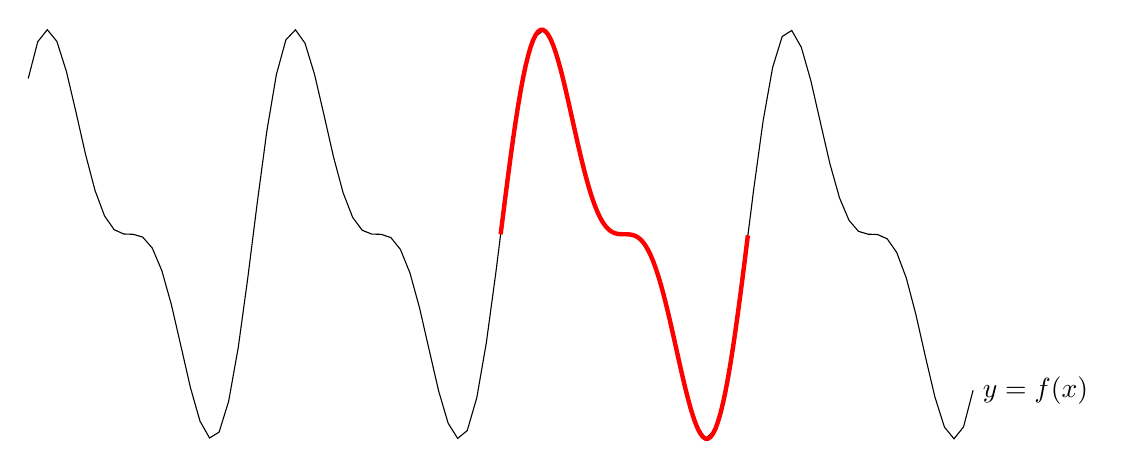
\begin{tikzpicture}
\YEaxis{8}{4}
\draw plot[samples=100,domain=-12:12](\x/2,{2*sin(\x r)+sin(2*\x r)}) node[right]{$y=f(x)$};
\draw[ultra thick, red] plot[samples=100,domain=0:6.28](\x/2,{2*sin(\x r)+sin(2*\x r)});
\end{tikzpicture}\end{center}

Additionally, $f(x)$ is odd. In a function with odd symmetry, if we mirror the right-hand portion of the curve (the portion to the right of the $y$-axis) across both the $y$-axis and the $x$-axis, it lines up with the left-hand portion of the curve.
\begin{center}\begin{tikzpicture}
\YEaxis{6}{4}
\draw plot[samples=100,domain=0:12](\x/2,{2*sin(\x r)+sin(2*\x r)}) node[right]{$y=f(x)$};
\draw[dashed] plot[samples=100,domain=-12:0](\x/2,{-2*sin(\x r)-sin(2*\x r)});
\draw (-3,-3) node{reflected across $y$-axis};
\end{tikzpicture}


\begin{tikzpicture}
\draw (0,1) node{};
\draw (0,-3) node{};
\draw[ultra thick, ->] (0,0)--(0,-2);
\end{tikzpicture}

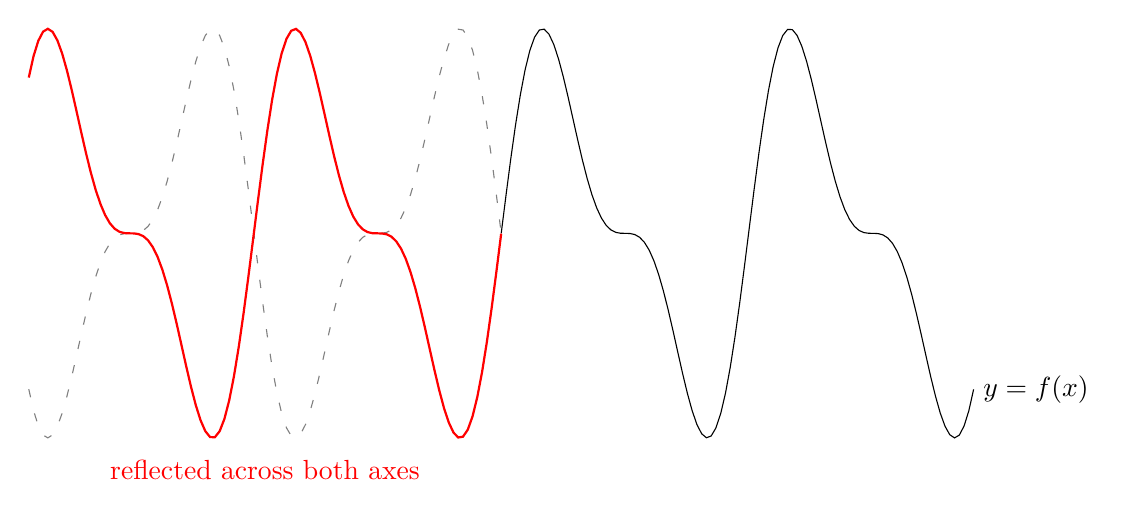
\begin{tikzpicture}
\YEaxis{6}{4}
\draw plot[samples=100,domain=0:12](\x/2,{2*sin(\x r)+sin(2*\x r)}) node[right]{$y=f(x)$};
\draw[loosely dashed, gray] plot[samples=100,domain=-12:0](\x/2,{-2*sin(\x r)-sin(2*\x r)});
\draw[red, thick] plot[samples=100,domain=-12:0](\x/2,{2*sin(\x r)+sin(2*\x r)});
\draw[red] (-3,-3) node{reflected across both axes};
\end{tikzpicture}
\end{center}
Since reflecting the right-hand portion of the graph across the $y$-axis, then the $x$-axis, gives us $f(x)$, we conclude $f(x)$ is odd.
\end{solution}


\begin{question}
Suppose $f(x)$ is an even function defined for all real numbers. Below is the curve $y=f(x)$ when $x>0$. Complete the sketch of the curve.
\begin{center}\begin{tikzpicture}
\YEaxis{6}{4}
\draw plot[domain=0:6, samples=100](\x,{cos(\x r)+\x^2/12-1});
\end{tikzpicture}\end{center}
\end{question}
\begin{hint}
Since the function is even, you only have to reflect the portion shown across the $y$-axis to complete the sketch.
\end{hint}
\begin{answer}
\begin{center}\begin{tikzpicture}
\YEaxis{6}{4}
\draw plot[domain=0:6, samples=100](\x,{cos(\x r)+\x^2/12-1});
\draw plot[domain=0:6, samples=100](-\x,{cos(\x r)+\x^2/12-1});
\end{tikzpicture}\end{center}
\end{answer}
\begin{solution}
Since the function is even, we simply reflect the portion shown across the $y$-axis to complete the sketch.
\begin{center}\begin{tikzpicture}
\YEaxis{6}{4}
\draw plot[domain=0:6, samples=100](\x,{cos(\x r)+\x^2/12-1});
\draw plot[domain=0:6, samples=100](-\x,{cos(\x r)+\x^2/12-1});
\end{tikzpicture}\end{center}
\end{solution}


\begin{Mquestion}
Suppose $f(x)$ is an odd function defined for all real numbers. Below is the curve $y=f(x)$ when $x>0$. Complete the sketch of the curve.
\begin{center}\begin{tikzpicture}
\YEaxis{6}{4}
\draw plot[domain=0:6, samples=100](\x,{cos(\x r)+\x^2/12-1});
\end{tikzpicture}\end{center}
\end{Mquestion}
\begin{hint}
Since the function is odd, to complete the sketch, reflect the portion shown across the $y$-axis, then the $x$-axis.
\end{hint}
\begin{answer}
\begin{center}\begin{tikzpicture}
\YEaxis{6}{4}
\draw plot[domain=0:6, samples=100](\x,{cos(\x r)+\x^2/12-1});
\draw plot[domain=0:6, samples=100](-\x,{-cos(\x r)-\x^2/12+1});
\end{tikzpicture}\end{center}
\end{answer}
\begin{solution}
Since the function is odd, to complete the sketch, we reflect the portion shown across the $y$-axis (shown dashed), then the $x$-axis (shown in red).
\begin{center}\begin{tikzpicture}
\YEaxis{6}{4}
\draw plot[domain=0:6, samples=100](\x,{cos(\x r)+\x^2/12-1});
\draw[loosely dashed] plot[domain=0:6, samples=100](-\x,{cos(\x r)+\x^2/12-1});
\draw[red] plot[domain=0:6, samples=100](-\x,{-cos(\x r)-\x^2/12+1});
\end{tikzpicture}
\end{center}
\end{solution}

%%%%%%%%%%%%%%%%%%
\subsection*{\Procedural}
%%%%%%%%%%%%%%%%%%


\begin{Mquestion}
\[f(x)=\frac{x^4-x^6}{e^{x^2}}\]
Show that $f(x)$ is even.
\end{Mquestion}
\begin{hint}
A function is even if $f(-x)=f(x)$.
\end{hint}
\begin{answer}
A function is even if $f(-x)=f(x)$.
\begin{align*}
f(-x)&=\frac{(-x)^4-(-x)^6}{e^{(-x)^2}}\\
&=\frac{x^4-x^6}{e^{x^2}}\\
&=f(x)
\end{align*}
So, $f(x)$ is even.
\end{answer}
\begin{solution}
A function is even if $f(-x)=f(x)$.
\begin{align*}
f(-x)&=\frac{(-x)^4-(-x)^6}{e^{(-x)^2}}\\
&=\frac{x^4-x^6}{e^{x^2}}\\
&=f(x)
\end{align*}
So, $f(x)$ is even.
\end{solution}


\begin{question}
\[f(x)=\sin(x)+\cos\left(\frac{x}{2}\right)\]
Show that $f(x)$ is periodic.
\end{question}
\begin{hint}
Its period is not $2\pi$.
\end{hint}
\begin{answer}
For any real number $x$, we will show that $f(x)=f(x+4\pi)$.
\begin{align*}
f(x+4\pi)&=\sin(x+4\pi)+\cos\left(\frac{x+4\pi}{2}\right)\\
&=\sin(x+4\pi)+\cos\left(\frac{x}{2}+2\pi\right)\\
&=\sin(x)+\cos\left(\frac{x}{2}\right)\\
&=f(x)
\end{align*}
So, $f(x)$ is periodic.
\end{answer}
\begin{solution}
For any real number $x$, we will show that $f(x)=f(x+4\pi)$.
\begin{align*}
f(x+4\pi)&=\sin(x+4\pi)+\cos\left(\frac{x+4\pi}{2}\right)\\
&=\sin(x+4\pi)+\cos\left(\frac{x}{2}+2\pi\right)\\
&=\sin(x)+\cos\left(\frac{x}{2}\right)\\
&=f(x)
\end{align*}
So, $f(x)$ is periodic.
\end{solution}


\Instructions{In Questions~\ref{s3.6.4eqfirst} through \ref{s3.6.4eqlast}, find the symmetries of a function from its equation.}

\begin{Mquestion}\label{s3.6.4eqfirst}
\[f(x)=x^4+5x^2+\cos\left(x^3\right)\]
What symmetries (even, odd, periodic) does $f(x)$ have?
\end{Mquestion}
\begin{hint}
Simplify $f(-x)$ to see whether it is the same as $f(x)$, $-f(x)$, or neither.
\end{hint}
\begin{answer}
even
\end{answer}
\begin{solution}
$f(x)$ is not periodic. (You don't really have to justify this, but if you wanted to, you could say something like this. Notice $f(0)=1$. Whenever $x>10$, $f(x)>1$. Then the value of $f(0)$ is \emph{not} repeated indefinitely, so $f(x)$ is not periodic.)

To decide whether $f(x)$ is even, odd, or neither, simplify $f(-x)$:
\begin{align*}
f(-x)&=(-x)^4+5(-x)^2+\cos\left((-x)^3\right)\\
&=x^4+5x^2+\cos(-x^3)\\
&=x^4+5x^2+\cos(x^3)\\
&=f(x)
\end{align*}
Since $f(-x)=f(x)$, our function is even.
\end{solution}

\begin{question}
\[f(x)=x^5+5x^4\]
What symmetries (even, odd, periodic) does $f(x)$ have?
\end{question}
\begin{hint}
Simplify $f(-x)$ to see whether it is the same as $f(x)$, $-f(x)$, or neither.
\end{hint}
\begin{answer}
none
\end{answer}
\begin{solution}
It should be clear that $f(x)$ is not periodic.  (If you wanted to justify this, you could note that $f(x)=0$ has exactly two solutions, $x=0,\,-{5}$. Since the value of $f(0)$ is repeated only twice, and not indefinitely, $f(x)$ is not periodic.)

To decide whether $f(x)$ is odd, even, or neither, we simplify $f(-x)$.
\begin{align*}
f(-x)&=(-x)^5+5(-x)^{4}\\
&=-x^5+5x^4\\
\end{align*}
We see that  $f(-x)$ is not equal to $f(x)$ or to $-f(x)$.
For instance, when $x=1$:
\begin{itemize}
\item $f(-x)=f(-1)=4$,
\item $f(x)=f(1)=6$, and
\item $-f(x)=-f(1)=-6$. \end{itemize}
Since $f(-x)$ is not equal to $f(x)$ or to $-f(x)$, $f(x)$ is neither even nor odd.
\end{solution}


\begin{question}
\[f(x)=\tan\left(\pi x\right)\]
 What is the period of $f(x)$?
\end{question}
\begin{hint}
Find the smallest value $k$ such that $f(x+k)=f(x)$ for any $x$ in the domain of $f$.

You may use the fact that the period of $g(X)=\tan X$ is $\pi$.
\end{hint}
\begin{answer}
1
\end{answer}
\begin{solution}
Recall the period of $g(X)=\tan X $ is $\pi$.
\begin{align*}
\tan(X+\pi)&=\tan(X)&&\mbox{for any $X$ in the domain of $\tan X$}
\intertext{Replacing $X$ with $\pi x$:}
\tan(\pi x + \pi)&=\tan(\pi x)&&\mbox{for any $x$ in the domain of $\tan(\pi x)$}\\
\tan(\pi(x+1))&=\tan(\pi x)&&\mbox{for any $x$ in the domain of $\tan(\pi x)$}\\
f(x+1)&=f(x)&&\mbox{for any $x$ in the domain of $\tan(\pi x)$}
\end{align*}
The period of $f(x)$ is 1.
\end{solution}



%%%%%%%%%%%%%%%%%%
\subsection*{\Application}
%%%%%%%%%%%%%%%%%%


\begin{question}\label{s3.6.4eqlast}
\[f(x)=\tan\left(3 x\right)+\sin\left(4 x\right)\]
What is the period of $f(x)$?
\end{question}
\begin{hint}
It is true that $f(x)=f(x+2\pi)$ for every $x$ in the domain of $f(x)$, but the period is not $2\pi$.
\end{hint}
\begin{answer}
$\pi$
\end{answer}
\begin{solution}
Let's consider $g(x)=\tan(3x)$ and $h(x)=\sin(4x)$ separately. Recall that $\pi$ is the period of tangent.
\begin{align*}
\tan X &= \tan(X+\pi)&&\mbox{for every $X$ in the domain of $\tan X$}
\intertext{Replacing $X$ with $3x$:}
\tan(3x)&=\tan(3x+\pi)&&\mbox{for every $x$ in the domain of $\tan 3x$}\\
\tan(3x)&=\tan\left(3\left(x+\frac{\pi}{3}\right)\right)&&\mbox{for every $x$ in the domain of $\tan 3x$}\\
g(x)&=g\left(x+\frac{\pi}{3}\right)&&\mbox{for every $x$ in the domain of $\tan 3x$}
\intertext{So, the period of $g(x)=\tan(3x)$ is $\dfrac{\pi}{3}$.}
\intertext{Similarly, $2\pi$ is the period of sine.}
\sin(X)&=\sin(X+2\pi)&&\mbox{for every $X$ in the domain of  $\sin(X)$}
\intertext{Replacing $X$ with $4x$:}
\sin(4x)&=\sin(4x+2\pi)&&\mbox{for every $x$ in the domain of  $\sin(4x)$}\\
\sin(4x)&=\sin\left(4\left(x+\frac{\pi}{2}\right)\right)&&\mbox{for every $x$ in the domain of  $\sin(4x)$}\\
h(x)&=h\left(x+\frac{\pi}{2}\right)&&\mbox{for every $x$ in the domain of  $\sin(4x)$}
\end{align*}
So, the period of $h(x)=\sin(4x)$ is $\dfrac{\pi}{2}$.

All together, $f(x)=g(x)+h(x)$ will repeat when both $g(x)$ and $h(x)$ repeat. The least common integer multiple of $\dfrac{\pi}{3}$ and $\dfrac{\pi}{2}$ is $\pi$. Since $g(x)$ repeats every $\dfrac{\pi}{3}$ units, and $h(x)$ repeats every $\dfrac{\pi}{2}$ units, they will not both repeat until we move $\pi$ units. So, the period of $f(x)$ is $\pi$.
\end{solution}
